\begin{standout}[第〇章]
    绪论\\
    Introduction
\end{standout}

\begin{frame}{大纲}
    \setbeamertemplate{section in toc}[sections numbered]
    \begin{multicols}{2}
        \tableofcontents
    \end{multicols}
\end{frame}

\section{课程简介}

\begin{frame}{\insertsectionhead}
    \begin{figure}
        \centering
        \begin{tikzpicture}
            \pie[rotate=0, polar, explode=0.2,
                % color={cyan!30!black,yellow!30!black,magenta!30!black,white!30!black}
                color={gray}
            ]{
                15/课堂讨论与测验,
                15/在线学习,
                20/实验报告,
                50/期末考试
            }
        \end{tikzpicture}
        \caption{总成绩构成}
        \label{fig:score_composition}
    \end{figure}
\end{frame}

\begin{frame}{\insertsectionhead}
    \begin{block}{先修课程}
        \begin{itemize}
            \item 编程语言:Python/C
            \item 数学:初等数学
        \end{itemize}
    \end{block}

    \begin{block}{后继课程}
        \begin{itemize}
            \item 操作系统、计算机网络、数据库等
            \item 计算机图形学、图像与视频处理等
            \item 游戏开发技术、游戏引擎技术、移动应用开发等
        \end{itemize}
    \end{block}
\end{frame}

\section{数据结构简介}

\subsection{何为数据结构}

\begin{frame}{\insertsubsectionhead}
    \begin{quote}\raggedright
        ``In solving a problem with or without a computer it is necessary to choose an abstraction of reality, i.e., \alert{to define a set of data that is to represent the real situation}. "\\
        \vspace{2ex}
        \small
        \raggedleft — Niklaus E. Wirth\\
        \raggedleft Algorithms and Data Structures, 1985, p11.
    \end{quote}
\end{frame}

\begin{frame}{\insertsubsectionhead}
    \Large \[
        \text{程序设计}=\underbrace{\text{数据结构}}_\text{\alert{载体}}+\underbrace{\text{算法}}_\text{\alert{灵魂}}
    \]
\end{frame}

\begin{frame}{\insertsubsectionhead}
    \begin{exampleblock}{实例:如何在书架上摆放图书}
        \begin{itemize}
            \item 寻求解决问题的方法,与数据规模有关
            \item 大规模数据背景下,更关注解决问题的效率
        \end{itemize}
    \end{exampleblock}
    \pause
    \begin{exampleblock}{需考虑的因素}
        \begin{itemize}
            \item 插入:如何插入新书?
            \item 检索:如何查找旧书?
        \end{itemize}
    \end{exampleblock}
\end{frame}

\begin{fragile}
    \frametitle{\insertsubsectionhead}
    \bicolumns[0.5]{
        \begin{block}{方法一:随便放}
            \pause
            \begin{itemize}
                \item 插入:哪里有空放哪里
                \item 检索:崩溃!!
            \end{itemize}
        \end{block}
        \pause
        \begin{block}{方法二:按书名拼音顺序}
            \pause
            \begin{itemize}
                \item 插入:先检索,再插入
                \item 检索:二分
            \end{itemize}
        \end{block}
        \pause
    }{
        \begin{block}{方法三:先分区,每区内按方法二处理}
            \pause
            \begin{itemize}
                \item 插入:先检索,再插入
                \item 检索:先定区,再二分
            \end{itemize}
        \end{block}
        \pause
        \begin{alertblock}{问题}
            \begin{itemize}
                \item 图书如何分类?区域大小如何确定?
                \item 二分法如何实现?
            \end{itemize}
        \end{alertblock}
    }
\end{fragile}

\begin{standout}[\insertsubsectionhead]
    解决问题方法的效率与\alert{数据的组织方式}有关
\end{standout}

\begin{fragile}
    \frametitle{\insertsubsectionhead}
    \begin{columns}[t]
        \column{0.33\textwidth}
        \begin{block}{方法一:随便放}
            \begin{center}
                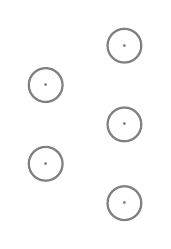
\begin{tikzpicture}[ >=stealth, thick, black!50, %
                        list item/.style={draw=gray, circle, thick} %
                    ]
                    \node [list item] (item1) at (0.5,1) {.}; %
                    \node [list item] (item2) at (-0.5,0.5) {.}; %
                    \node [list item] (item3) at (0.5,0) {.}; %
                    \node [list item] (item4) at (-0.5,-0.5) {.}; %
                    \node [list item] (item5) at (0.5,-1) {.}; %
                \end{tikzpicture}
            \end{center}
        \end{block}
        \pause
        \column{0.33\textwidth}
        \begin{block}{方法二:按序放}
            \begin{center}
                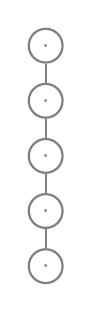
\begin{tikzpicture}[ >=stealth, thick, black!50, %
                        list item/.style={draw=gray, circle, thick} %
                    ]
                    \node [list item] (item1) at (0,1.4) {.}; %
                    \node [list item] (item2) at (0,0.7) {.}; %
                    \node [list item] (item3) at (0,0) {.}; %
                    \node [list item] (item4) at (0,-0.7) {.}; %
                    \node [list item] (item5) at (0,-1.4) {.}; %
                    \draw  (item1) -- (item2) -- (item3) -- (item4) -- (item5); %
                \end{tikzpicture}
            \end{center}
        \end{block}
        \pause
        \column{0.33\textwidth}
        \begin{block}{方法三:分类按序放}
            \begin{center}
                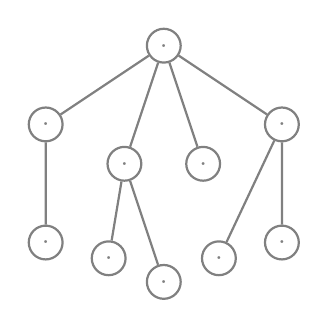
\begin{tikzpicture}[ >=stealth, thick, black!50, %
                        list item/.style={draw=gray, circle, thick} %
                    ]
                    \node [list item] (item1) at (0,1) {.}; %
                    \node [list item] (item2) at (-1.5,0) {.}; %
                    \node [list item] (item3) at (-0.5,-0.5) {.}; %
                    \node [list item] (item4) at (0.5,-0.5) {.}; %
                    \node [list item] (item5) at (1.5,0) {.}; %
                    \node [list item] (item6) at (-1.5,-1.5) {.}; %
                    \node [list item] (item7) at (-0.7,-1.7) {.}; %
                    \node [list item] (item8) at (0,-2) {.}; %
                    \node [list item] (item9) at (0.7,-1.7) {.}; %
                    \node [list item] (item10) at (1.5,-1.5) {.}; %
                    \draw  (item1) -- (item2) -- (item6); %
                    \draw  (item1) -- (item3) -- (item7); %
                    \draw  (item3) -- (item8); %
                    \draw  (item1) -- (item4); %
                    \draw  (item5) -- (item9); %
                    \draw  (item1) -- (item5) -- (item10); %
                \end{tikzpicture}
            \end{center}
        \end{block}
    \end{columns}
    \pause
    \begin{columns}[t]
        \column{0.33\textwidth}
        \begin{center}
            集合结构
        \end{center}
        \pause
        \column{0.33\textwidth}
        \begin{center}
            线性结构
        \end{center}
        \pause
        \column{0.33\textwidth}
        \begin{center}
            树形结构
        \end{center}
        \pause
    \end{columns}
    \vspace{4ex}
    \begin{quote}
        由实际生活问题\alert{抽象}出计算机可解的数据结构
    \end{quote}
\end{fragile}

\begin{fragile}
    \frametitle{\insertsubsectionhead}
    \begin{block}{数据的\alert{逻辑结构}}
        \begin{itemize}
            \item 从具体问题中抽象出的\alert{数学模型}
            \item 对现实世界中某个特定领域知识或概念的\alert{抽象}
        \end{itemize}
    \end{block}
    \pause
    \begin{columns}[t]
        \column{0.2\textwidth}
        \begin{center}
            集合结构\\\vspace{2ex}
            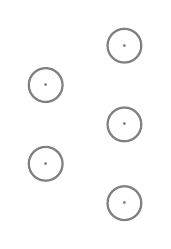
\begin{tikzpicture}[ >=stealth, thick, black!50, %
                    list item/.style={draw=gray, circle, thick} %
                ]
                \node [list item] (item1) at (0.5,1) {.}; %
                \node [list item] (item2) at (-0.5,0.5) {.}; %
                \node [list item] (item3) at (0.5,0) {.}; %
                \node [list item] (item4) at (-0.5,-0.5) {.}; %
                \node [list item] (item5) at (0.5,-1) {.}; %
            \end{tikzpicture}
        \end{center}
        \column{0.2\textwidth}
        \begin{center}
            线性结构$1:1$\\\vspace{2ex}
            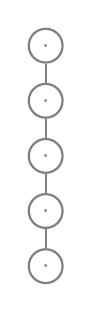
\begin{tikzpicture}[ >=stealth, thick, black!50, %
                    list item/.style={draw=gray, circle, thick} %
                ]
                \node [list item] (item1) at (0,1.4) {.}; %
                \node [list item] (item2) at (0,0.7) {.}; %
                \node [list item] (item3) at (0,0) {.}; %
                \node [list item] (item4) at (0,-0.7) {.}; %
                \node [list item] (item5) at (0,-1.4) {.}; %
                \draw  (item1) -- (item2) -- (item3) -- (item4) -- (item5); %
            \end{tikzpicture}
        \end{center}
        \column{0.25\textwidth}
        \begin{center}
            树形结构$1:n$\\\vspace{2ex}
            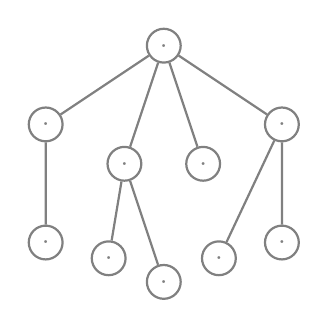
\begin{tikzpicture}[ >=stealth, thick, black!50, %
                    list item/.style={draw=gray, circle, thick} %
                ]
                \node [list item] (item1) at (0,1) {.}; %
                \node [list item] (item2) at (-1.5,0) {.}; %
                \node [list item] (item3) at (-0.5,-0.5) {.}; %
                \node [list item] (item4) at (0.5,-0.5) {.}; %
                \node [list item] (item5) at (1.5,0) {.}; %
                \node [list item] (item6) at (-1.5,-1.5) {.}; %
                \node [list item] (item7) at (-0.7,-1.7) {.}; %
                \node [list item] (item8) at (0,-2) {.}; %
                \node [list item] (item9) at (0.7,-1.7) {.}; %
                \node [list item] (item10) at (1.5,-1.5) {.}; %
                \draw  (item1) -- (item2) -- (item6); %
                \draw  (item1) -- (item3) -- (item7); %
                \draw  (item3) -- (item8); %
                \draw  (item1) -- (item4); %
                \draw  (item5) -- (item9); %
                \draw  (item1) -- (item5) -- (item10); %
            \end{tikzpicture}
        \end{center}
        \column{0.25\textwidth}
        \begin{center}
            图形结构$m:n$\\\vspace{2ex}
            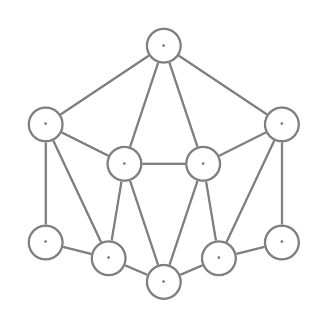
\begin{tikzpicture}[ >=stealth, thick, black!50, %
                    list item/.style={draw=gray, circle, thick} %
                ]
                \node [list item] (item1) at (0,1) {.}; %
                \node [list item] (item2) at (-1.5,0) {.}; %
                \node [list item] (item3) at (-0.5,-0.5) {.}; %
                \node [list item] (item4) at (0.5,-0.5) {.}; %
                \node [list item] (item5) at (1.5,0) {.}; %
                \node [list item] (item6) at (-1.5,-1.5) {.}; %
                \node [list item] (item7) at (-0.7,-1.7) {.}; %
                \node [list item] (item8) at (0,-2) {.}; %
                \node [list item] (item9) at (0.7,-1.7) {.}; %
                \node [list item] (item10) at (1.5,-1.5) {.}; %
                \draw  (item1) -- (item2) -- (item6) -- (item7) -- (item8) -- (item9) -- (item10); %
                \draw  (item2) -- (item3) -- (item4) -- (item5); %
                \draw  (item1) -- (item3) -- (item7); %
                \draw  (item3) -- (item8); %
                \draw  (item1) -- (item4) -- (item8); %
                \draw  (item5) -- (item9); %
                \draw  (item2) -- (item7); %
                \draw  (item4) -- (item9); %
                \draw  (item1) -- (item5) -- (item10); %
            \end{tikzpicture}
        \end{center}
    \end{columns}
\end{fragile}

\begin{fragile}
    \frametitle{\insertsubsectionhead}
    \begin{block}{数据的\alert{物理结构}}
        \begin{itemize}
            \item 数据的逻辑结构在计算机中的存储形式
            \item 同一逻辑结构可采用多种不同的物理结构表达
        \end{itemize}
    \end{block}
    \pause
    \begin{columns}
        \column{0.5\textwidth}
        \begin{center}
            顺序存储结构\\\vspace{2ex}
            
\begin{tikzpicture}[ >=stealth, thick, black!50, %
                    list item/.style={draw=gray, circle, thick} %
                ]
                \node [list item] (item0) at (-1.5,0) {.}; %
                \node [list item] (item1) at (-1,0) {.}; %
                \node [list item] (item2) at (-0.5,0) {.}; %
                \node [list item] (item3) at (0,0) {.}; %
                \node [list item] (item4) at (0.5,0) {.}; %
                \node [list item] (item5) at (1,0) {.}; %
                \node [list item] (item6) at (-1.5,0) {.}; %
            \end{tikzpicture}
        \end{center}
        \pause
        \column{0.5\textwidth}
        \begin{center}
            链式存储结构\\\vspace{2ex}
            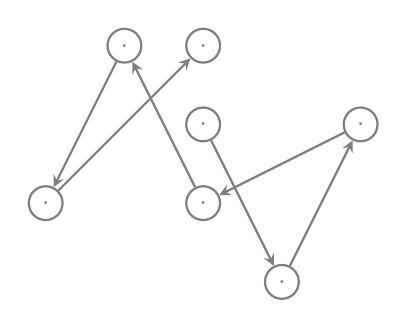
\begin{tikzpicture}[ >=stealth, thick, ->, black!50, %
                    list item/.style={draw=gray, circle, thick} %
                ]
                \node [list item] (item1) at (0,0) {.}; %
                \node [list item] (item2) at (1,-2) {.}; %
                \node [list item] (item3) at (2,0) {.}; %
                \node [list item] (item4) at (0,-1) {.}; %
                \node [list item] (item5) at (-1,1) {.}; %
                \node [list item] (item6) at (-2,-1) {.}; %
                \node [list item] (item7) at (0,1) {.}; %
                \draw  (item1) -- (item2); %
                \draw  (item2) -- (item3); %
                \draw  (item3) -- (item4); %
                \draw  (item4) -- (item5); %
                \draw  (item5) -- (item6); %
                \draw  (item6) -- (item7); %
            \end{tikzpicture}
        \end{center}
    \end{columns}
\end{fragile}

\begin{fragile}
    \frametitle{\insertsubsectionhead}
    \begin{exampleblock}{实例:编程实现按序打印正整数}
        \begin{itemize}
            \item 输入:正整数个数$n$
            \item 输出:按顺序打印从$1$至$n$的全部正整数
        \end{itemize}
    \end{exampleblock}
    \pause
    \bicolumns[0.5]{
        \begin{itemize}
            \item<2->迭代实现
            \begin{minted}{c}
                void print_n(int n) {
                    for (int i = 1; i <= n; ++i) {
                        printf("%d\n", i);
                    }
                }
            \end{minted}
        \end{itemize}
    }{
        \begin{itemize}
            \item<3-> 递归实现
                \begin{minted}{c}
                void print_n(int n) {
                    if (n) {
                        print_n(n - 1);
                        printf("%d\n", n);
                    }
                }
            \end{minted}
        \end{itemize}
    }
\end{fragile}

\begin{fragile}
    \frametitle{\insertsubsectionhead}
    \begin{exampleblock}{实例:编程实现按序打印正整数(续)}
        \vspace{2ex}
        \bicolumns[0.5]{
            \begin{itemize}
                \item 测试
                      \begin{minted}{c}
                    #include <stdio.h>
                    
                    void print_n(int);
                    
                    int main(void) {
                        int n;
                        scanf("%d", &n);
                        print_n(n);
                        return 0;
                    }
                \end{minted}
            \end{itemize}
        }{
            \begin{itemize}
                \item<2-> 当$n=10$时,二者均输出
                    \begin{minted}[linenos=false]{console}
                    1
                    2
                    3
                    4
                    5
                    6
                    7
                    8
                    9
                    10
                \end{minted}
            \end{itemize}
        }
    \end{exampleblock}
\end{fragile}

\begin{fragile}
    \frametitle{\insertsubsectionhead}
    \begin{exampleblock}{实例:编程实现按序打印正整数(续)}
        \vspace{2ex}
        \bicolumns[0.5]{
            \begin{itemize}
                \item 当$n=1,000,000$时,迭代版输出
                      \begin{minted}[linenos=false]{console}
                    ...
                    999992
                    999993
                    999994
                    999995
                    999996
                    999997
                    999998
                    999999
                    1000000
                \end{minted}
            \end{itemize}
        }{
            \begin{itemize}
                \item<2-> 递归版输出(GNU/Linux, GCC)
                    \begin{minted}[linenos=false]{console}
                    zsh: segmentation fault (core dumped) ...
                \end{minted}
                \item<3-> 递归版无输出(Windows, GCC)
                    \begin{minted}[linenos=false]{console}
                    
                \end{minted}
            \end{itemize}
        }
    \end{exampleblock}
\end{fragile}

\begin{standout}[\insertsubsectionhead]
    解决问题方法的效率与\alert{空间利用率}有关
\end{standout}

\begin{fragile}
    \frametitle{\insertsubsectionhead}
    \begin{exampleblock}{实例:求多项式值}
        \begin{itemize}
            \item 输入:多项式阶数$n$、系数序列$\{a_{k}\}_{k=0}^{n}$、给定点$v$
            \item 输出:多项式$f(x) = a_{0} + a_{1}x + \cdots + a_{n-1}x^{n-1} + a_{n}x^{n}$在点$v$处的值$f(v)$
            \item<2-> 常规实现
                \begin{minted}[highlightlines={4}]{c}
                double f(int n, double *a, double x) {
                    double p = a[0];
                    for (int i = 1; i <= n; ++i) {
                        p += a[i] * pow(x, i); // 采用标准库中的幂函数
                    }
                    return p;
                }
            \end{minted}
        \end{itemize}
    \end{exampleblock}
\end{fragile}

\begin{fragile}
    \frametitle{\insertsubsectionhead}
    \begin{exampleblock}{实例:求多项式值(续)}
        \begin{itemize}
            \item 考虑如下转换:
                  \begin{align*}
                      f(x) & = a_{0} + a_{1}x + \cdots + a_{n-1}x^{n-1} + a_{n}x^{n}  \\
                           & = a_{0} + x(a_{1} + x(\cdots(a_{n-1} + x(a_{n}))\cdots))
                  \end{align*}
            \item<2-> 换一种思路实现
                \begin{minted}[highlightlines={4}]{c}
                double f(int n, double *a, double x) {
                    double p = a[n];
                    for (int i = n - 1; i >= 0; --i) {
                        p = a[i] + x * p;
                    }
                    return p;
                }
            \end{minted}
        \end{itemize}
    \end{exampleblock}
\end{fragile}

\begin{fragile}
    \frametitle{\insertsubsectionhead}
    \begin{exampleblock}{实例:多项式求值(续)}
        \vspace{2ex}
        \bicolumns[0.55]{
            \begin{itemize}
                \item 测试运行时间\footnotemark
                      \begin{minted}{c}
                    void time_f(int times) {
                        const int N = 9; // 多项式阶数
                        double a[] = {
                            0, 1, 2, 3, 4, 5, 6, 7, 8, 9
                        }; // 多项式系数
                        clock_t start = clock(); // 开始计时
                        for (int i = 0; i < times; ++i) {
                            f(N, a, 1.1); // 重复执行测试函数
                        }
                        clock_t end = clock(); // 结束计时
                        double duration = (double)(end - start)
                                / CLK_TCK / times; // 取平均值
                        printf("%6.2e\n", duration);
                    }
                \end{minted}
            \end{itemize}
            \pause
        }{
            \begin{itemize}
                \item 执行$10^{7}$次取平均,结果分别为\vspace{2ex}
                      \small
                      \begin{tabular}{rl}
                          \toprule
                          \textbf{解决方案} & \textbf{运行时间(秒)}    \\
                          \midrule
                          常规实现          & $4.55\times10^{-7}$ \\
                          另一种思路         & $3.20\times10^{-8}$ \\
                          \bottomrule
                      \end{tabular}
            \end{itemize}
        }
    \end{exampleblock}
    \footnotetext{实现计时功能需包含\mintinline{console}{<time.h>}头文件}
\end{fragile}

\begin{standout}[\insertsubsectionhead]
    解决问题方法的效率与\alert{算法巧妙程度}有关
\end{standout}

\subsection{为何学数据结构}

\begin{standout}[\insertsubsectionhead]
    使人真正地会写程序
\end{standout}

\subsection{基本概念}

\begin{fragile}
    \frametitle{\insertsubsectionhead}
    \begin{block}{数据结构(Data Structures)}
        \begin{itemize}
            \item 一门研究\alert{非数值}问题中的操作对象及其间的\alert{关系}与\alert{操作}等相关问题的学科
        \end{itemize}
    \end{block}
    \pause
    \begin{exampleblock}{说明}
        \begin{itemize}
            \item<2-> \alert{数值}问题可由\alert{数学方程}解决
            \item<3-> 操作对象间的关系包括\alert{逻辑}关系与\alert{物理}关系
        \end{itemize}
    \end{exampleblock}
\end{fragile}

\begin{frame}
    \frametitle{\insertsubsectionhead}
    \begin{block}{数据(Data)}
        \begin{itemize}
            \item 描述客观事物的符号
            \item 计算机中可\alert{操作}的对象
            \item 可被计算机\alert{识别}、并输入给计算机\alert{处理}的符号集合
        \end{itemize}
    \end{block}
    \pause
    \begin{exampleblock}{例}
        \begin{itemize}
            \item 数值类型,如\alert{整型、浮点型}等
            \item 非数值类型,如\alert{字符型、图形、图像、音频、视频}等
        \end{itemize}
    \end{exampleblock}
\end{frame}

\begin{frame}{\insertsubsectionhead}
    \begin{block}{数据元素(Data Element)}
        \begin{itemize}
            \item 组成数据的、有一定意义的\alert{基本}单位
            \item 在计算机中通常作为\alert{整体}处理与考虑
            \item 又名:\textbf{元素(element)}、\textbf{结点(node)}、\textbf{顶点(vertex)}、\textbf{记录(record)}等
        \end{itemize}
    \end{block}
    \pause
    \begin{exampleblock}{例}
        \begin{itemize}
            \item 在人类中的\alert{人}
            \item 在畜类中的\alert{牛、马、羊、猪、狗、鸡、鸭}等
            \item 在学籍管理系统中一个学生的\alert{基本信息记录}
        \end{itemize}
    \end{exampleblock}
\end{frame}

\begin{frame}{\insertsubsectionhead}
    \begin{block}{数据项(Data Item)}
        \begin{itemize}
            \item 一个数据元素可由多个数据项组成
            \item 数据不可分割的\alert{最小}单位
        \end{itemize}
    \end{block}
    \pause
    \begin{exampleblock}{例}
        \begin{itemize}
            \item 人可有\alert{眼、耳、鼻、舌、身}等数据项
            \item 人亦可有\alert{姓名、性别、年龄、电话}等数据项
            \item 学生的基本信息记录中可有\alert{学号、姓名、性别}等数据项
        \end{itemize}
    \end{exampleblock}
\end{frame}

\begin{frame}{\insertsubsectionhead}
    \begin{block}{数据对象(Data Object)}
        \begin{itemize}
            \item \alert{性质相同}\footnotemark{}的数据元素的集合
            \item 数据的一类子集
        \end{itemize}
    \end{block}
    \pause
    \begin{exampleblock}{例}
        \begin{itemize}
            \item 包含若干名学生基本信息的\alert{基本信息表}
        \end{itemize}
    \end{exampleblock}
    \footnotetext{指所有数据元素具有相同\alert{数量}与\alert{类型}的数据项}
\end{frame}

\subsection{抽象数据类型}

\begin{frame}{\insertsubsectionhead}
    \begin{block}{逻辑层与物理层}
        \begin{itemize}
            \item 逻辑层:只需停留在使用层面,了解\alert{接口(interface)}即可
            \item 物理层:尚需深入至更深层次,需掌握其\alert{实现(implementation)}
        \end{itemize}
    \end{block}
    \pause
    \begin{table}[h]
        \small
        \centering
        \caption{逻辑层与物理层的实例}
        \begin{tabular}{cccc}
            \toprule
            \textbf{实例}                  & \textbf{角色} & \textbf{行为}             & \textbf{层次} \\
            \midrule
            \multirow{2}{*}{\textbf{汽车}} & 司机          & 上下车、油门、刹车、方向盘等          & 逻辑层         \\
                                         & 工程师         & 发动机、传动轴、刹车片等原理          & 物理层         \\
            \midrule
            \multirow{2}{*}{\textbf{电脑}} & 文员          & 编辑文档、收发邮件、影音娱乐等         & 逻辑层         \\
                                         & 科学家         & 数据结构、操作系统、体系结构、计算机组成等原理 & 物理层         \\
            \bottomrule
        \end{tabular}
        \label{tab:log_phy}
    \end{table}
\end{frame}

\begin{frame}{\insertsubsectionhead}
    \begin{block}{数据类型(Data Type)}
        \begin{itemize}
            \item 一组性质相同的值的\alert{集合}、及在该集合上定义的一些\alert{操作}的总称
        \end{itemize}
    \end{block}
    \pause
    \begin{block}{抽象(Abstract)}
        \begin{itemize}
            \item 抽取出事物具有的\alert{普遍性}的本质
        \end{itemize}
    \end{block}
    \pause
    \begin{block}{抽象数据类型(Abstract Data Type, ADT)}
        \begin{itemize}
            \item 对已有数据类型的抽象
            \item 只描述数据类型\alert{是什么},而非如何实现
            \item 仅取决于\alert{逻辑特性},与其在计算机内部的表示与实现\footnotemark{}无关
        \end{itemize}
    \end{block}
    \footnotetext<3>{包括:数据存储的硬件环境、物理结构,实现操作的算法、编程语言等}
\end{frame}

\begin{frame}{\insertsubsectionhead}
    \begin{quote}
        \textbf{抽象数据类型}实现了数据的\alert{逻辑层}与\alert{物理层}的分离
    \end{quote}
    \pause
    \begin{table}[h]
        \small
        \centering
        \caption{抽象数据类型作用举例}
        \begin{tabular}{rcc}
            \toprule
                                        & \textbf{电动车}             & \textbf{燃油车} \\
            \midrule
            \textbf{能源与动力(\alert{物理层})} & 电能驱动                     & 汽油燃烧供能驱动     \\
            \textbf{驾驶方式(\alert{逻辑层})}  & \multicolumn{2}{c}{基本类似}                \\
            \bottomrule
        \end{tabular}
        \label{tab:ele_gas}
    \end{table}
\end{frame}

\begin{fragile}
    \frametitle{\insertsubsectionhead}
    \begin{columns}
        \column{0.4\textwidth}
        \begin{block}{描述ADT的一般形式}
            \begin{minted}[linenos=false]{sh}
                抽象数据类型名称 {
                数据:
                    数据对象及其间逻辑关系的定义
                操作:
                    操作1名称
                        初始条件描述
                        操作结果描述
                        ...
                    操作2名称
                        ...
                    ...
                    操作n名称
                        ...
                }
            \end{minted}
        \end{block}
        \pause
        \column{0.6\textwidth}
        \begin{exampleblock}{例:矩阵ADT}
            \begin{minted}[linenos=false,escapeinside=《》]{c}
                    Matrix {
                    数据:
                        三元组{a,i,j}, 《$A=(a_{i,j})_{i\in[1,m],j\in[1,n]}$\footnotemark》
                    操作:
                        Matrix create(int m, int n):
                            根据输入创建并返回《$m\times n$》阶空矩阵
                        int rows(Matrix A):
                            获取并返回矩阵《$A$》的行数
                        int columns(Matrix A):
                            获取并返回矩阵《$A$》的列数
                        ElementType get_entry(int i, int j):
                            根据输入获取并返回矩阵元素《$a_{i,j}$》
                        ...
                    }
                \end{minted}
        \end{exampleblock}
    \end{columns}
    \footnotetext{与具体实现无关,可以数组、链表或其他任何合理结构实现}
\end{fragile}

\section{算法简介}

\subsection{何为算法}

\begin{frame}{\insertsubsectionhead}
    \begin{block}{算法(Algorithm)}
        \begin{itemize}
            \item 解决特定问题求解步骤的描述,表现为指令的有限序列每条指令表示一个或多个操作
        \end{itemize}
    \end{block}
\end{frame}

\begin{fragile}
    \frametitle{\insertsubsectionhead}
    \begin{block}{算法的伪码描述}
        \begin{itemize}
            \item 与硬件环境、物理结构、编程语言等无关的一种指令集描述
        \end{itemize}
    \end{block}
    \pause
    \begin{exampleblock}{例:Euclid辗转相除法求最大公约数}
        \begin{algorithmx}[alg:euclid]{Euclid算法}
            \Procedure{Euclid}{$a,b$}\Comment{$a$与$b$的最大公约数}
            \State $r\gets a\bmod b$
            \While{$r\neq 0$}\Comment{若$r=0$则可跳出循环返回答案}
            \State $a\gets b$
            \State $b\gets r$
            \State $r\gets a\bmod b$
            \EndWhile\label{euclidendwhile}
            \State \textbf{return} $b$\Comment{最大公约数为$b$}
            \EndProcedure
        \end{algorithmx}
    \end{exampleblock}
\end{fragile}

\subsection{算法特点}

\begin{frame}{\insertsubsectionhead}
    \begin{block}{算法五大特性}
        \begin{itemize}
            \item 输入(Input):有$n$个输入,其中$n\in\mathbb{Z}^{+}\cup\{0\}$
            \item 输出(Output):有$m$个输出,其中$m\in\mathbb{Z}^{+}$
            \item 有穷性(Finiteness):在执行\alert{有限步}后、且在可接受时间内结束,而非陷入无限循环
            \item 确定性(Definiteness):每个步骤均有\alert{明确含义},避免出现歧义
            \item 可行性(Feasibility):可被现有计算机\alert{实现},而非仅存于理论研究中
        \end{itemize}
    \end{block}
\end{frame}

\begin{frame}{\insertsubsectionhead}
    \begin{block}{算法设计的要求}
        \begin{itemize}
            \item 正确性(Correctness):无歧义,能正确反映问题要求,并得到正确答案
            \item 可读性(Readability):便于人类理解与交流
            \item 健壮性(Robustness):能正确处理不合法输入,而非产生异常或莫名其妙结果
            \item 高效性(Efficiency):占用尽可能少的时间与空间
        \end{itemize}
    \end{block}
\end{frame}

\begin{frame}{\insertsubsectionhead}
    \begin{block}{衡量算法效率的指标}
        \begin{itemize}
            \item 时间复杂度$T(n)$:当问题规模为$n$时,算法中核心语句的总执行次数$T(n)$
            \item 空间复杂度$S(n)$:当问题规模为$n$时,执行算法核心步骤所占用的存储空间$S(n)$
        \end{itemize}
    \end{block}
    \pause
    \begin{exampleblock}{说明}
        \begin{itemize}
            \item 二者均只与问题规模$n$有关,与硬件等其他条件无关
            \item 二者均越小越好,但往往不可得兼
        \end{itemize}
    \end{exampleblock}
\end{frame}

\subsection{算法分析}

\begin{frame}{\insertsubsectionhead}
    \begin{block}{算法的渐进分析(Asymptotic Analysis)}
        \begin{itemize}
            \item 小规模问题往往无法反映算法的真实情况
            \item 着眼\alert{长远}、更注重时间复杂度总体变化\alert{趋势}与增长速度的策略与方法
        \end{itemize}
    \end{block}
\end{frame}

\begin{frame}{\insertsubsectionhead}
    \begin{block}{渐进上界:大$\mathcal{O}$记号}
        \begin{itemize}
            \item 若存在常数$c>0$、正整数$N$与函数$f(n)$,使得对任意满足$n>N$的$n$均有
                  \[
                      T(n) \leq cf(n),
                  \]
                  则称$f(n)$给出$T(n)$增长速度的一个\alert{渐进上界},记作$T(n)=\mathcal{O}(f(n))$
        \end{itemize}
    \end{block}
\end{frame}

\begin{frame}{\insertsubsectionhead}
    \begin{exampleblock}{渐进上界的性质}
        \begin{itemize}
            \item 对任意常数$c>0$,有
                  \[
                      \mathcal{O}(f(n))=\mathcal{O}(cf(n))
                  \]
            \item 对任意常数$a>b>0$,有
                  \[
                      \mathcal{O}(n^{a}+n^{b})=\mathcal{O}(n^{a})
                  \]
            \item 若$T_{f}(n)=\mathcal{O}(f(n))$且$T_{g}(n)=\mathcal{O}(g(n))$,则有
                  \begin{align*}
                      T_{f}(n)+T_{g}(n)       & =\max\{\mathcal{O}(f(n)),\mathcal{O}(g(n))\} \\
                      T_{f}(n)\cdot{}T_{g}(n) & =\mathcal{O}(f(n)\cdot{}g(n))
                  \end{align*}
        \end{itemize}
    \end{exampleblock}
\end{frame}

\begin{frame}{\insertsubsectionhead}
    \begin{table}[h]
        \small
        \centering
        \caption{常见渐进上界}
        \begin{tabular}{c|rrrrrr}
            \toprule
            \multirow{2}{*}{\textbf{渐进上界}} & \multicolumn{6}{c}{\textbf{输入规模}}                                                                       \\
                                           & $1$                               & $2$ & $4$  & $8$      & $16$                & $32$                  \\
            \midrule
            $\mathcal{O}(1)$               & $1$                               & $1$ & $1$  & $1$      & $1$                 & $1$                   \\
            $\mathcal{O}(\log_{2}n)$       & $0$                               & $1$ & $2$  & $3$      & $4$                 & $5$                   \\
            $\mathcal{O}(n)$               & $1$                               & $2$ & $4$  & $8$      & $16$                & $32$                  \\
            $\mathcal{O}(n\log_{2}n)$      & $0$                               & $2$ & $8$  & $24$     & $64$                & $160$                 \\
            $\mathcal{O}(n^{2})$           & $1$                               & $4$ & $16$ & $64$     & $256$               & $1,024$               \\
            $\mathcal{O}(n^{3})$           & $1$                               & $8$ & $64$ & $512$    & $4,096$             & $32,768$              \\
            \midrule
            $\mathcal{O}(2^{n})$           & $2$                               & $4$ & $16$ & $256$    & $65,536$            & $4,294,967,296$       \\
            $\mathcal{O}(n!)$              & $1$                               & $2$ & $24$ & $40,326$ & $2,092,278,988,000$ & $2.6313\times10^{37}$ \\
            \bottomrule
        \end{tabular}
        \label{tab:asymptotic_upper_bound}
    \end{table}
\end{frame}

\subsection{算法实例}

\begin{frame}{\insertsubsectionhead}
    \begin{exampleblock}{实例:求最大子序列和}
        \begin{itemize}
            \item 给定整数序列$\{a_{k}\}_{k=0}^{n-1}$,求其中连续子序列和
                  \[
                      s(i,j)=\sum_{k=i}^{j}{a_{k}}
                  \]
                  的最大值$s^{*}=\max_{0\leq{}i\leq{}j<n}{s(i,j)}$
        \end{itemize}
    \end{exampleblock}
    \pause
    \begin{exampleblock}{示范样例}
        \begin{itemize}
            \item 输入:$4,-3,5,-2,-1,2,6,-2$
            \item 输出\footnotemark{}:$11$
        \end{itemize}
    \end{exampleblock}
    \only<2>\footnotetext{注意到$4-3+5-2-1+2+6=11$}
\end{frame}

\begin{fragile}
    \frametitle{\insertsubsectionhead}
    \bicolumns[0.65]{
        \begin{block}{解决方案甲:直接解法}
            \begin{minted}[highlightlines={3,4,6}]{c}
                int max_subsequence_sum(int *a, int n) {
                    int max_sum = 0;
                    for (int i = 0; i < n; ++i) { // 子列左端
                        for (int j = i; j < n; ++j) { // 子列右端
                            int this_sum = 0;
                            for (int k = i; k <= j; ++k) { // 遍历子列
                                this_sum += a[k];
                            }
                            if (this_sum > max_sum) {
                                max_sum = this_sum; // 更新最值
                            }
                        }
                    }
                    return max_sum;
                }
            \end{minted}
        \end{block}
        \pause
    }{
        \begin{alertblock}{问题与改进}
            \begin{itemize}
                \item 三重循环
                \item $T(n)=\mathcal{O}(n^{3})$\pause
                \item 内层循环冗余
                \item 可与中层循环合并
            \end{itemize}
        \end{alertblock}
    }
\end{fragile}

\begin{fragile}
    \frametitle{\insertsubsectionhead}
    \bicolumns[0.65]{
        \begin{block}{解决方案乙:一种改进}
            \begin{minted}[highlightlines={3,5}]{c}
                int max_subsequence_sum(int *a, int n) {
                    int max_sum = 0;
                    for (int i = 0; i < n; ++i) { // 子列左端
                        int this_sum = 0;
                        for (int j = i; j < n; ++j) { // 遍历子列
                            this_sum += a[j];
                            if (this_sum > max_sum) {
                                max_sum = this_sum; // 更新最值
                            }
                        }
                    }
                    return max_sum;
                }
            \end{minted}
        \end{block}
        \pause
    }{
        \begin{alertblock}{问题与改进}
            \begin{itemize}
                \item 二重循环
                \item $T(n)=\mathcal{O}(n^{2})$\pause
                \item 能否更快
            \end{itemize}
        \end{alertblock}
    }
\end{fragile}

\begin{fragile}
    \frametitle{\insertsubsectionhead}
    \begin{block}{解决方案丙:分而治之}
        \begin{itemize}
            \item 将原问题逐步\alert{分解}为规模更小且更易解决的同类型子问题
            \item 将已解决的若干小问题逐步反向\alert{合并}为更简单的原问题
            \item 代码详见教材
        \end{itemize}
    \end{block}
\end{fragile}

\begin{fragile}
    \frametitle{\insertsubsectionhead}
    \begin{exampleblock}{解决方案丙的时间复杂度推导}
        \begin{itemize}
            \item 若问题规模为$n$,且\alert{分解}方式采用二分,单次\alert{合并}
                  操作耗时为$c$,则有
                  \begin{align*}
                      T(n) & = 2T\left(\frac{n}{2}\right) + nc                                \\
                           & = 2\left(2T\left(\frac{n}{2^{2}}\right) + \frac{n}{2}c\right)+nc \\
                           & \cdots                                                           \\
                           & \leq 2^{k}T\left(\frac{n}{2^{k}}\right) + knc,
                  \end{align*}
            \item<2-> 若$T(1)=\mathcal{O}(1)$,则当$k=\log_{2}{n}$时,有
                \[
                    T(n) = \mathcal{O}(n\log_{2}{n})
                \]
        \end{itemize}
    \end{exampleblock}
\end{fragile}

\begin{fragile}
    \frametitle{\insertsubsectionhead}
    \begin{figure}
        \centering
        \begin{bytefield}{1}
            \bitbox[]{6}{}\bitboxes[]{3}{{\tiny$0$}{\tiny$1$}{\tiny$2$}{\tiny$3$}{\tiny$4$}{\tiny$5$}{\tiny$6$}{\tiny$7$}} \\
            \bitbox[]{6}{\raggedleft\mintinline{c}{a}$\;\,$}\bitboxes{3}{{$+4$}{$-3$}{$+5$}{$-2$}{$-1$}{$+2$}{$+6$}{$-2$}} \\
            \bitbox[]{6}{\raggedleft$1:\;\,$}\only<2->{\bitbox{3}{\alert<2-3>{$+4$}}}\only<3->{\bitbox{3}{$-3$}}\only<4->{\bitbox{3}{\alert<4-7>{$+5$}}}\only<5->{\bitbox{3}{$-2$}}\only<6->{\bitbox{3}{$-1$}}\only<7->{\bitbox{3}{$+2$}}\only<8->{\bitbox{3}{\alert<8-14>{$+6$}}}\only<9->{\bitbox{3}{$-2$}} \\
            \bitbox[]{6}{\raggedleft$2:\;\,$}\only<10->{\bitbox{3}{$+4$}}\bitbox[]{3}{}\only<11->{\bitbox{3}{$+5$}}\bitbox[]{3}{}\bitbox[]{3}{}\only<12->{\bitbox{3}{$+2$}}\only<13->{\bitbox{3}{$+6$}}\bitbox[]{3}{} \\
            \bitbox[]{6}{\raggedleft$4:\;\,$}\only<14->{\bitbox{9}{$+6$}}\bitbox[]{6}{}\only<15->{\bitbox{6}{\alert<15>{$+8$}}}\bitbox[]{3}{} \\
            \bitbox[]{6}{\raggedleft$8:\;\,$}\only<16->{\bitbox{21}{\alert<16->{$+11$}}}\bitbox[]{3}{} \\
        \end{bytefield}
        \caption{解决方案丙示例演示过程}
        \label{fig:demo_3}
    \end{figure}
\end{fragile}

\begin{fragile}
    \frametitle{\insertsubsectionhead}
    \bicolumns[0.65]{
        \begin{block}{解决方案丁:在线处理}
            \begin{minted}[highlightlines={4}]{c}
                int max_subsequence_sum(int *a, int n) {
                    int max_sum = 0;
                    int this_sum = 0;
                    for (int j = 0; j < n; ++j) { // 遍历子列
                        this_sum += a[j];
                        if (this_sum > max_sum) {
                            max_sum = this_sum; // 更新最值
                        } else if (this_sum < 0) {
                            this_sum = 0; // 丢弃负子序列和
                        }
                    }
                    return max_sum;
                }
            \end{minted}
        \end{block}
        \pause
    }{
        \begin{alertblock}{问题与改进}
            \begin{itemize}
                \item 一重循环
                \item $T(n)=\mathcal{O}(n)$\pause
                \item 能否更快
            \end{itemize}
        \end{alertblock}
    }
\end{fragile}

\begin{fragile}
    \frametitle{\insertsubsectionhead}
    \begin{figure}
        \centering
        \begin{bytefield}{1}
            \bitbox[]{6}{}\bitboxes[]{3}{{\tiny$0$}{\tiny$1$}{\tiny$2$}{\tiny$3$}{\tiny$4$}{\tiny$5$}{\tiny$6$}{\tiny$7$}} \\
            \bitbox[]{6}{\raggedleft\mintinline{c}{a}$\;\,$}\bitboxes{3}{{\alert<2->{$+4$}}{\alert<3->{$-3$}}{\alert<4->{$+5$}}{\alert<5->{$-2$}}{\alert<6->{$-1$}}{\alert<7->{$+2$}}{\alert<8->{$+6$}}{\alert<9->{$-2$}}} \\
            \bitbox[]{6}{}\bitboxes[]{3}{{\only<2->{$\checkmark$}}{\only<4->{$\checkmark$}}{\only<4->{$\checkmark$}}{\only<8->{$\checkmark$}}{\only<8->{$\checkmark$}}{\only<8->{$\checkmark$}}{\only<8->{$\checkmark$}}{}} \\
            \bitbox[]{6}{\raggedleft\mintinline{c}{this_sum}$\;\,$}\bitbox{3}{\only<1>{$0$}\only<2>{$4$}\only<3>{$1$}\only<4>{$6$}\only<5>{$4$}\only<6>{$3$}\only<7>{$5$}\only<8>{$11$}\only<9>{$9$}} \\
            \bitbox[]{6}{\raggedleft\mintinline{c}{max_sum}$\;\,$}\bitbox{3}{\only<1>{$0$}\only<2-3>{$4$}\only<4-7>{$6$}\only<8->{$11$}} \\
        \end{bytefield}
        \caption{解决方案丁示例A演示过程}
        \label{fig:demo_4_a}
    \end{figure}
\end{fragile}

\begin{fragile}
    \frametitle{\insertsubsectionhead}
    \begin{figure}
        \centering
        \begin{bytefield}{1}
            \bitbox[]{6}{}\bitboxes[]{3}{{\tiny$0$}{\tiny$1$}{\tiny$2$}{\tiny$3$}{\tiny$4$}{\tiny$5$}{\tiny$6$}{\tiny$7$}} \\
            \bitbox[]{6}{\raggedleft\mintinline{c}{a}$\;\,$}\bitboxes{3}{{\alert<2->{$-1$}}{\alert<3->{$+3$}}{\alert<4->{$-2$}}{\alert<5->{$+4$}}{\alert<6->{$-6$}}{\alert<7->{$+1$}}{\alert<8->{$+6$}}{\alert<9->{$-1$}}} \\
            \bitbox[]{6}{}\bitboxes[]{3}{{}{\only<3-7>{$\checkmark$}}{\only<5-7>{$\checkmark$}}{\only<5-7>{$\checkmark$}}{}{\only<8->{$\checkmark$}}{\only<8->{$\checkmark$}}{}} \\
            \bitbox[]{6}{\raggedleft\mintinline{c}{this_sum}$\;\,$}\bitbox{3}{\only<1>{$0$}\only<2>{$0$}\only<3>{$3$}\only<4>{$1$}\only<5>{$5$}\only<6>{$0$}\only<7>{$1$}\only<8>{$7$}\only<9>{$6$}} \\
            \bitbox[]{6}{\raggedleft\mintinline{c}{max_sum}$\;\,$}\bitbox{3}{\only<1-2>{$0$}\only<3-4>{$3$}\only<5-7>{$5$}\only<8->{$7$}} \\
        \end{bytefield}
        \caption{解决方案丁示例B演示过程}
        \label{fig:demo_4_b}
    \end{figure}
\end{fragile}

\begin{frame}
    \frametitle{\insertsubsectionhead}
    \begin{alertblock}{解决方案丁的说明}
        \begin{itemize}
            \item 只需遍历一次序列即可求出结果
            \item 在任意时刻算法均可对截至当前子序列给出正确解
        \end{itemize}
    \end{alertblock}
\end{frame}

\begin{fragile}
    \frametitle{\insertsubsectionhead}
    \begin{table}[h]
        \centering
        \caption{各种解决方案运行时间比较(单位:秒)}
        \begin{tabular}{rl|ccccc}
            \toprule
            \multirow{2}{*}{\textbf{算法}} & \multirow{2}{*}{$T(n)$}     & \multicolumn{5}{c}{\textbf{输入规模}$n$}                                                 \\
                                         &                             & $10$                                 & $10^{2}$  & $10^{3}$  & $10^{4}$  & $10^{5}$  \\
            \midrule
            甲                            & $\mathcal{O}(n^{3})$        & $0.00103$                            & $0.47015$ & $448.77$  & $\infty$  & $\infty$  \\
            乙                            & $\mathcal{O}(n^{2})$        & $0.00045$                            & $0.01112$ & $1.1233$  & $111.13$  & $\infty$  \\
            丙                            & $\mathcal{O}(n\log_{2}{n})$ & $0.00066$                            & $0.00486$ & $0.05843$ & $0.68631$ & $8.0113$  \\
            丁                            & $\mathcal{O}(n)$            & $0.00034$                            & $0.00063$ & $0.00333$ & $0.03042$ & $0.29823$ \\
            \bottomrule
        \end{tabular}
        \label{tab:max_subsequence_sum_timing}
    \end{table}
\end{fragile}

\section{如何学数据结构与算法}

\begin{standout}[\insertsubsectionhead]
    掌握原理,多加练习
\end{standout}

\subsection{推荐的参考资料}

\begin{frame}{\insertsubsectionhead}
    \begin{columns}
        \column{0.5\textwidth}
        \vspace{4ex}
        \begin{figure}
            \centering
            
\includegraphics[height=0.6\textheight]{images/cheng2020dahua.jpg}
            \caption{大话数据结构\cite{cheng2020dahua}}
            \label{fig:cheng20200dahua}
        \end{figure}
        \column{0.5\textwidth}
        \begin{itemize}
            \item 通俗易懂
            \item 适合入门
        \end{itemize}
    \end{columns}
\end{frame}

\begin{frame}{\insertsubsectionhead}
    \begin{columns}
        \column{0.5\textwidth}
        \vspace{4ex}
        \begin{figure}
            \centering
            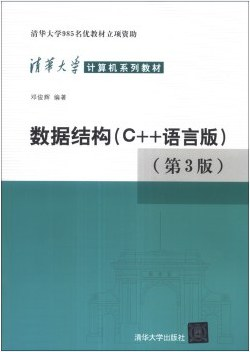
\includegraphics[height=0.6\textheight]{images/deng2013data.jpg}
            \caption{数据结构(C++版)\cite{deng2013data}}
            \label{fig:deng2013data}
        \end{figure}
        \column{0.5\textwidth}
        \begin{itemize}
            \item 脉络清晰
            \item 适合入门与进阶
            \item 可免费获取几乎所有资源
        \end{itemize}
    \end{columns}
\end{frame}

\begin{frame}{\insertsubsectionhead}
    \begin{columns}
        \column{0.5\textwidth}
        \vspace{4ex}
        \begin{figure}
            \centering
            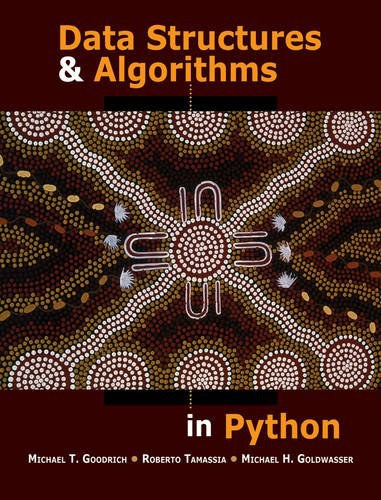
\includegraphics[height=0.6\textheight]{images/goodrich2013data.jpg}
            \caption{数据结构与算法(Python版)\cite{goodrich2013data}}
            \label{fig:goodrich2013data}
        \end{figure}
        \column{0.5\textwidth}
        \begin{itemize}
            \item 概念解释较为透彻
            \item 适合入门
            \item 翻译欠佳,建议原版
        \end{itemize}
    \end{columns}
\end{frame}

\begin{frame}{\insertsubsectionhead}
    \begin{columns}
        \column{0.5\textwidth}
        \vspace{4ex}
        \begin{figure}
            \centering
            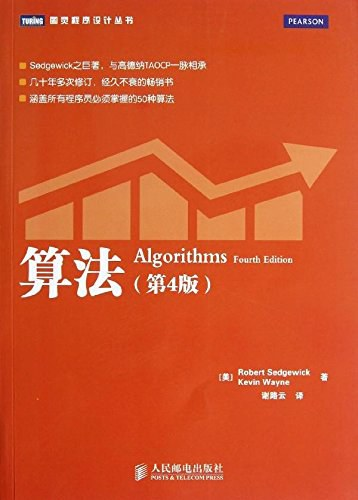
\includegraphics[height=0.6\textheight]{images/sedgewick2011algorithms.jpg}
            \caption{算法\cite{sedgewick2011algorthims}}
            \label{fig:sedgewick2011algorithms}
        \end{figure}
        \column{0.5\textwidth}
        \begin{itemize}
            \item 循序渐进
            \item 适合入门
            \item 可配合教学视频
        \end{itemize}
    \end{columns}
\end{frame}

\begin{frame}{\insertsubsectionhead}
    \begin{columns}
        \column{0.5\textwidth}
        \vspace{4ex}
        \begin{figure}
            \centering
            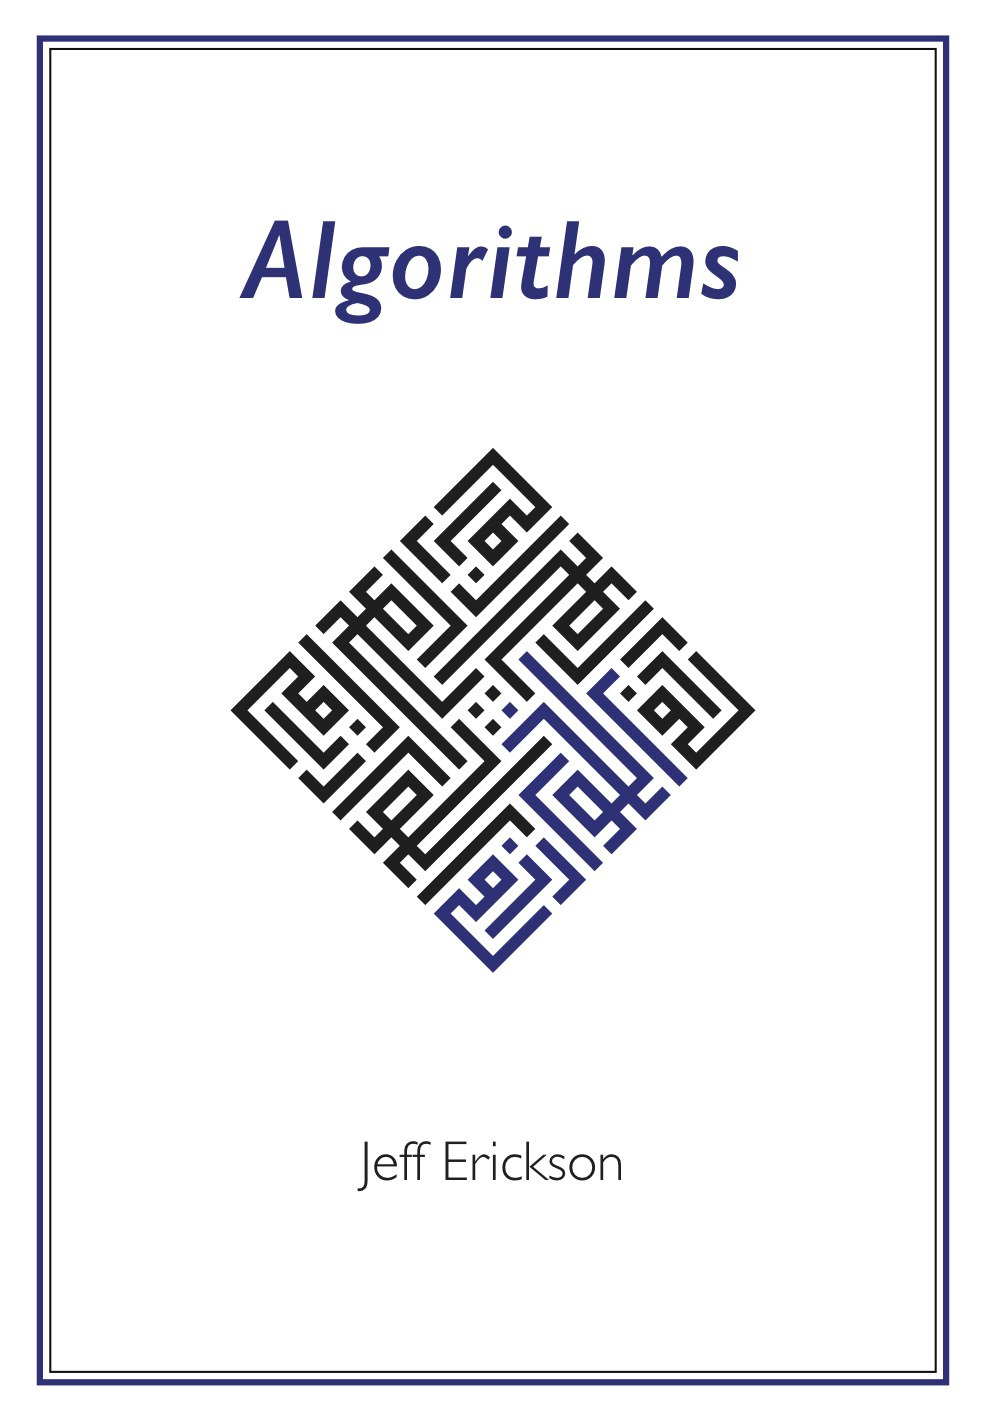
\includegraphics[height=0.6\textheight]{images/jeff2019algorithms.jpg}
            \caption{算法\cite{jeff2019algorithms}}
            \label{fig:jeff2019algorithms}
        \end{figure}
        \column{0.5\textwidth}
        \begin{itemize}
            \item 可读性极高
            \item 算法进阶之作
            \item 开源免费
        \end{itemize}
    \end{columns}
\end{frame}

\begin{frame}{\insertsubsectionhead}
    \begin{columns}
        \column{0.5\textwidth}
        \vspace{4ex}
        \begin{figure}
            \centering
            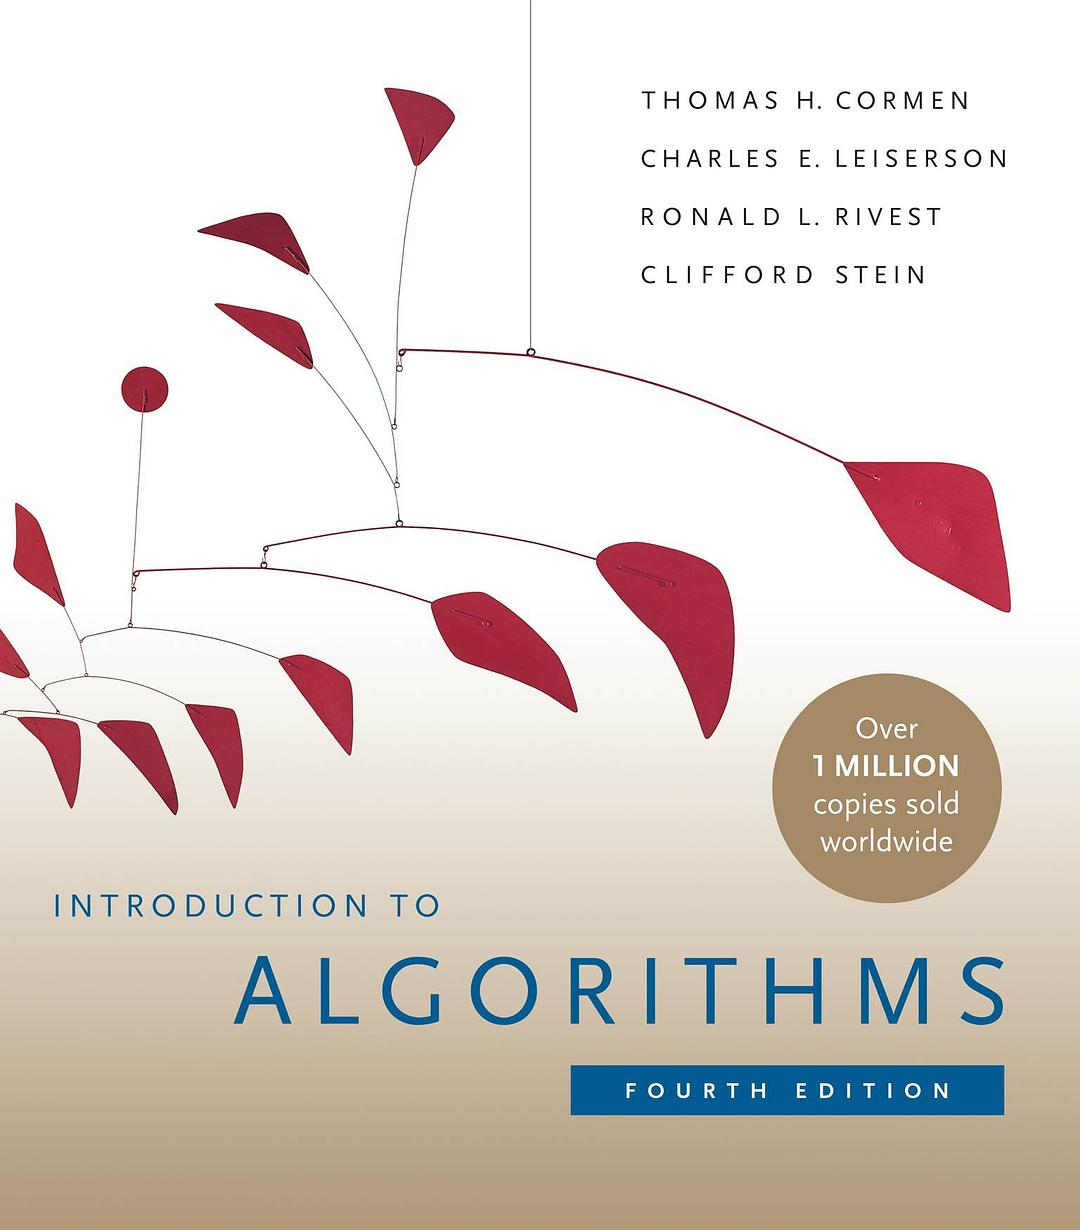
\includegraphics[height=0.6\textheight]{images/cormen2022introduction.jpg}
            \caption{算法导论\cite{cormen2022introduction}}
            \label{fig:cormen2022introduction}
        \end{figure}
        \column{0.5\textwidth}
        \begin{itemize}
            \item 算法介绍全面深刻
            \item 与编程语言无关
            \item 领域权威
        \end{itemize}
    \end{columns}
\end{frame}

\begin{frame}{\insertsubsectionhead}
    \begin{columns}
        \column{0.5\textwidth}
        \vspace{4ex}
        \begin{figure}
            \centering
            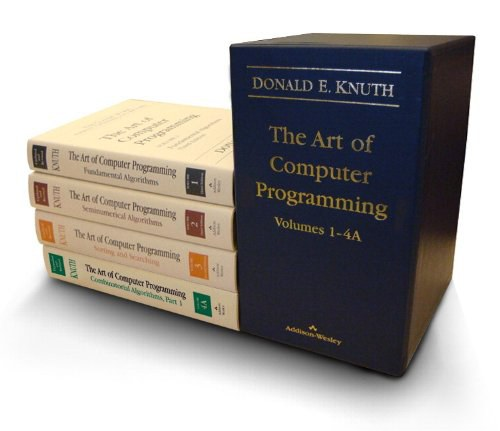
\includegraphics[height=0.6\textheight]{images/taocp.jpg}
            \caption{计算机程序设计艺术\cite{knuth1997art}}
            \label{fig:knuth1997art}
        \end{figure}
        \column{0.5\textwidth}
        \begin{itemize}
            \item 计算机科学领域圣经级著作
            \item 高德纳(Donald E. Knuth)毕生力作
            \item 数据结构开山之作
        \end{itemize}
    \end{columns}
\end{frame}

\section{小结}

\begin{frame}
    \frametitle{\insertsectionhead}
    \begin{itemize}
        \item 数据结构为程序设计的\alert{载体},算法是程序设计的\alert{灵魂}
        \item 解决问题方法的效率与\alert{数据的组织方式}、\alert{空间利用率}以及
        \alert{算法的巧妙程度}有关
        \item 数据结构研究\alert{非数值}问题中对象的操作及其间的关系
        \item 数据结构有\alert{逻辑结构}与\alert{物理结构}两大分类方式
        \item 抽象数据类型实现了逻辑层与物理层的分离
        \item 算法描述解决特定问题步骤,表现为指令的有限序列,每条指令表示一个或
        多个操作
        \item 算法五大特性:输入、输出、有穷、确定、可行
        \item 衡量算法效率的指标包括\alert{空间}与\alert{时间}复杂度
        \item 算法的渐进分析着眼长远、注重时间复杂度的\alert{总体变化趋势}与增长
        速度的策略与方法
    \end{itemize}
\end{frame}

\begin{standout}[]
    问与答
\end{standout}

\appendix

\section{附录}

\begin{frame}[allowframebreaks]{参考文献}
    \bibliography{references}
    \bibliographystyle{alpha}
\end{frame}